\documentclass[hyperref={pdfpagelabels=false}]{beamer}
%\fontfamily{phv}\selectfont
\usepackage{ucs}
\usepackage[utf8x]{inputenc}
\usepackage[T1]{fontenc}
\usepackage[ngerman]{babel}

\usepackage{url}
\usepackage{etoolbox}
\appto\UrlBreaks{\do\a\do\b\do\c\do\d\do\e\do\f\do\g\do\h\do\i\do\j
\do\k\do\l\do\m\do\n\do\o\do\p\do\q\do\r\do\s\do\t\do\u\do\v\do\w
\do\x\do\y\do\z\do\-}

\usepackage{caption}

\usepackage{pgfplots}

\usepackage{tikz}
\usepackage{lmodern}
\title{Hintergrundsegmentierung}   
\author{Christian Tanzer\\Jonas Bühlmeyer} 
\date{15. März 2017} 



\begin{document}

\begin{frame}
	\maketitle
\end{frame}

\setcounter{framenumber}{0}
\addtobeamertemplate{navigation symbols}{}{
\usebeamerfont{footline}
\usebeamercolor[blue]{footline}
\hspace{1em}
\insertframenumber/\inserttotalframenumber
}

\begin{frame}[t]{Inhaltsverzeichnis}
	\tableofcontents[] 
\end{frame}


\title{Self-Balanced SENsitivity SEgmenter}   
\author{Jonas Bühlmeyer} 
\date{}

\section{Self-Balanced SENsitivity SEgmenter}

\begin{frame}
	\maketitle
\end{frame}



\begin{frame}[t]{Konzept des Algorithmus}
	\begin{figure}
		\centering
		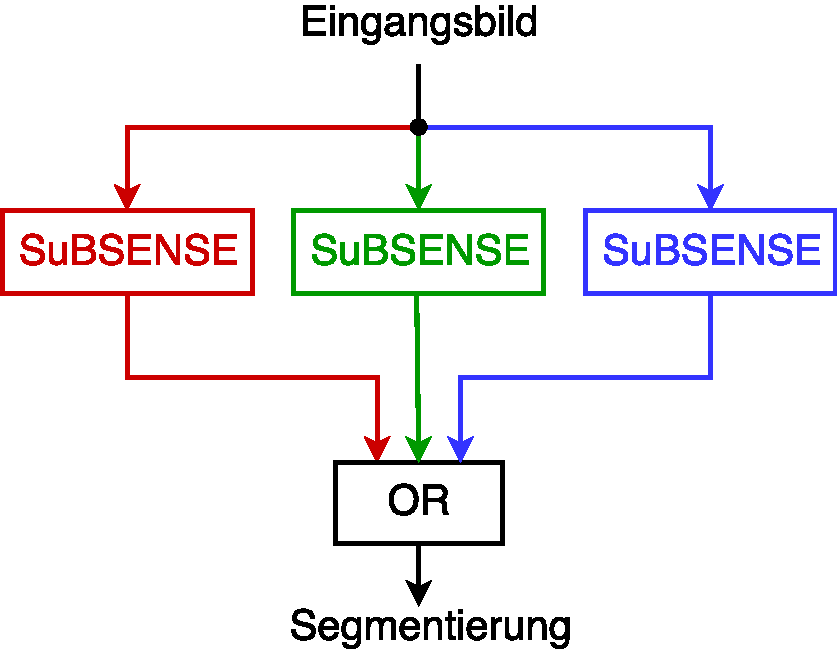
\includegraphics[width=0.8\linewidth]{Abbildungen/multiprocess.pdf}
		\label{fig:Abbildungen/Grid}
	\end{figure}
\end{frame}

\begin{frame}[t]{Konzept des Algorithmus}
	\bigskip
	\bigskip
	\bigskip 
	\begin{figure}
		\centering
		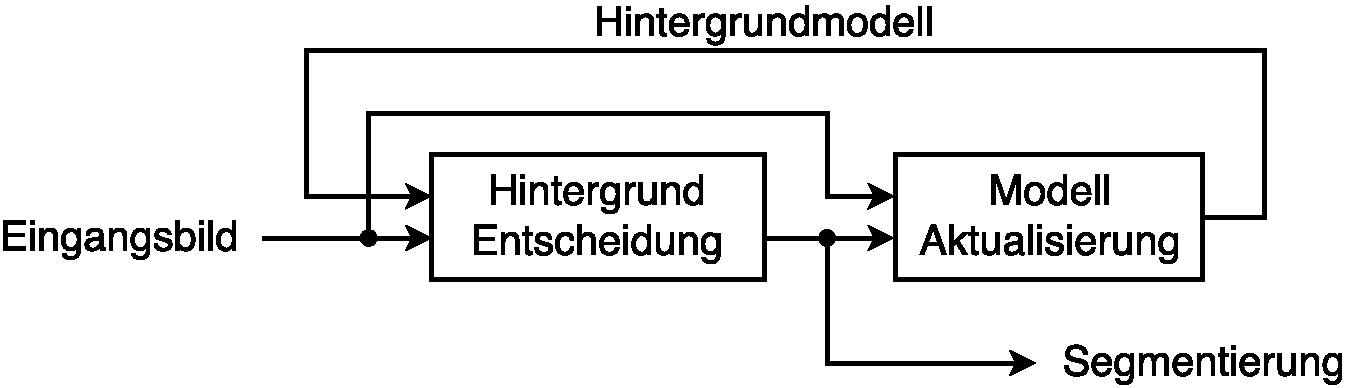
\includegraphics[width=1\linewidth]{Abbildungen/gesamt.pdf}
		\label{fig:Abbildungen/Grid}
	\end{figure}
\end{frame}


\begin{frame}[t]{Konzept des Algorithmus -- Hintergrundentscheidung}
	\begin{figure}
		\centering
		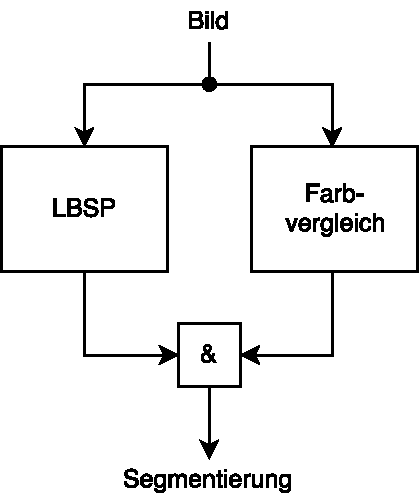
\includegraphics[width=0.6\linewidth]{Abbildungen/Konzept.pdf}
		\label{fig:Abbildungen/Grid}
	\end{figure}
\end{frame}



\begin{frame}[t]{Farbvergleich -- Entscheidung }
	\bigskip
	\bigskip
	\bigskip


	\begin{equation*}
		S_t(x)= \left\{
				\begin{array}{ll} 
					1, &  \# (I_t(x) - B_n(x) < R, \forall n) < \# min\\
					0, & sonst
				\end{array}
			\right .
	\end{equation*}
\end{frame}

\begin{frame}[t]{Farbvergleich -- Vergleich der Farbwerte}
	\bigskip
	\bigskip
	\bigskip

	\begin{figure}
		\centering
		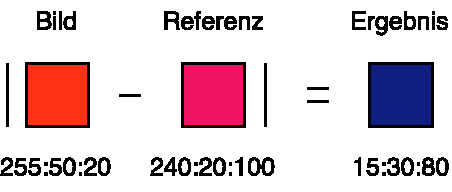
\includegraphics[width=0.6\linewidth]{Abbildungen/Farb_Vergleich.pdf}
		\label{fig:Abbildungen/Grid}
	\end{figure}
	\centering
	\bigskip
	$\Rightarrow$ die Farbwerte werden durch Subtraktion mit der Referenz verglichen
\end{frame}

\begin{frame}[t]{Farbvergleich -- Vergleich der Farbwerte}
	\centering
	\bigskip
	\bigskip
	\bigskip
	15 $<$ R$_{color} \rightarrow$ 1

	\bigskip
	30 $>$ R$_{color} \rightarrow$ 0
	
	\bigskip
	80 $>$ R$_{color} \rightarrow$ 0

	\bigskip
	\bigskip
	$\Rightarrow$ einmal pro Referenzwert im Hintergrundmodell
	\bigskip
	
	$\Rightarrow$ Anzahl der 1 pro Pixel größer als minimal Anzahl
	\bigskip
	
	$\Rightarrow$ Vordergrund
\end{frame}


\begin{frame}[t]{Farbvergleich -- Beispiel}
	\vspace{1.65em}
	\begin{figure}
		\centering
		\begin{minipage}{0.45\linewidth}
			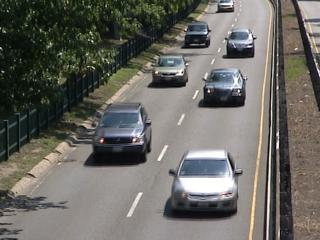
\includegraphics[width=1\linewidth]{Abbildungen/Eingang3.jpg}
			\caption*{Eingangsbild}
		\end{minipage}
		\begin{minipage}{0.45\linewidth}
			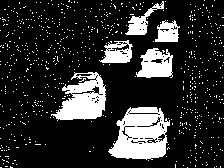
\includegraphics[width=1\linewidth]{Abbildungen/color_decision.jpg}
			\caption*{Farbvergleich Segmentierung}
		\end{minipage}
	\end{figure}
\end{frame}


\begin{frame}[t]{Konzept des Algorithmus}
	\begin{figure}
		\centering
		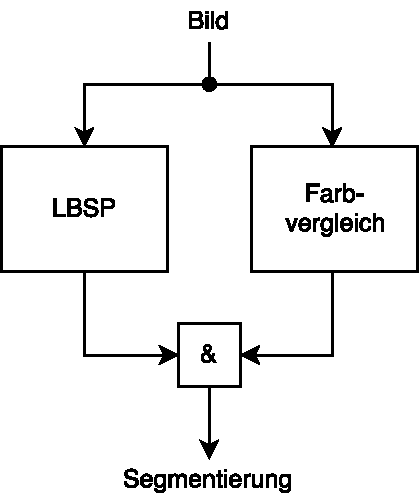
\includegraphics[width=0.6\linewidth]{Abbildungen/Konzept.pdf}
		\label{fig:Abbildungen/Grid}
	\end{figure}
\end{frame}


\begin{frame}[t]{LBSP -- Raster}
	\centering
	\begin{figure}
		\centering
		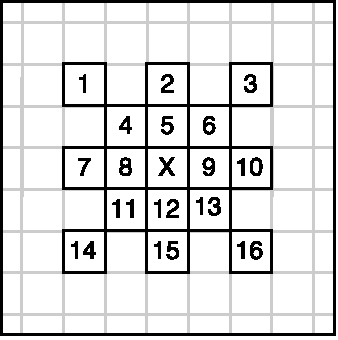
\includegraphics[width=0.45\linewidth]{Abbildungen/Grid.pdf}
		\label{fig:Abbildungen/Grid}
	\end{figure}

\end{frame}

\begin{frame}[t]{LBSP -- Vergleich der Farbwerte}
	\bigskip
	\bigskip
	\bigskip

	\begin{figure}
		\centering
		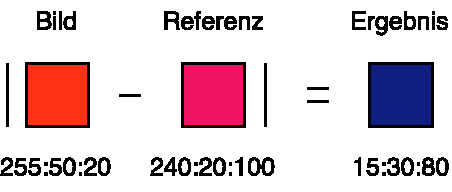
\includegraphics[width=0.6\linewidth]{Abbildungen/Farb_Vergleich.pdf}
		\label{fig:Abbildungen/Grid}
	\end{figure}
	\centering
	\bigskip
	$\Rightarrow$ die Farbwerte werden durch Subtraktion mit der Referenz verglichen
\end{frame}


\begin{frame}[t]{LBSP -- Vergleich der Farbwerte}
	\centering
	\bigskip
	\bigskip
	\bigskip
	15 $<$ R$_{lbsp} \rightarrow$ 0

	\bigskip
	30 $>$ R$_{lbsp} \rightarrow$ 1
	
	\bigskip
	80 $>$ R$_{lbsp} \rightarrow$ 1

	\bigskip
	\bigskip
	$\Rightarrow$ einmal pro Referenzwert im Raster
	\bigskip
	
	$\Rightarrow$ Referenz: 1 1 1 0\quad1 1 1 1\quad 0 0 1 1\quad 1 1 1 1

\end{frame}


\begin{frame}[t]{LBSP -- Vergleich der Pattern}
	\centering
	\begin{table}
		\centering
		\label{tab:label}
		\renewcommand{\arraystretch}{2}
		\begin{tabular}{lc}
			Referenz& 	1 1 1 0\quad 1 1 1 1\quad 0 0 1 1\quad 1 1 1 1\\
			Pixel 1& 	1 1 0 0\quad 1 1 1 1\quad 0 0 1 1\quad 1 0 0 0\\
			& 		$\Rightarrow$ 12/16 $\rightarrow$ Hintergrund\\
			Pixel 2& 	0 0 0 0\quad 1 0 1 1\quad 0 1 0 0\quad 0 0 0 1\\
			& 		$\Rightarrow$ 5/16 $\rightarrow$ Vordergrund\\
		\end{tabular}
	\end{table}
\end{frame}

\begin{frame}[t]{LBSP -- Beispiel}
	\vspace{1.65em}
	\begin{figure}
		\centering
		\begin{minipage}{0.45\linewidth}
			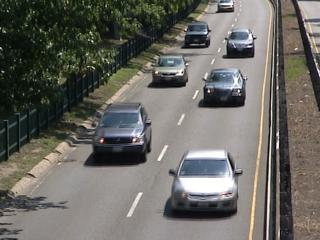
\includegraphics[width=1\linewidth]{Abbildungen/Eingang3.jpg}
			\caption*{Eingangsbild}
		\end{minipage}
		\begin{minipage}{0.45\linewidth}
			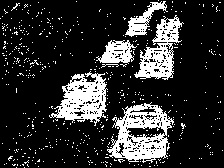
\includegraphics[width=1\linewidth]{Abbildungen/lbsp_decision.jpg}
			\caption*{LBSP Segmentierung}
		\end{minipage}
	\end{figure}
\end{frame}



\begin{frame}[t]{Hintergrundmodell}
	\bigskip
	\bigskip
	\begin{figure}
		\centering
		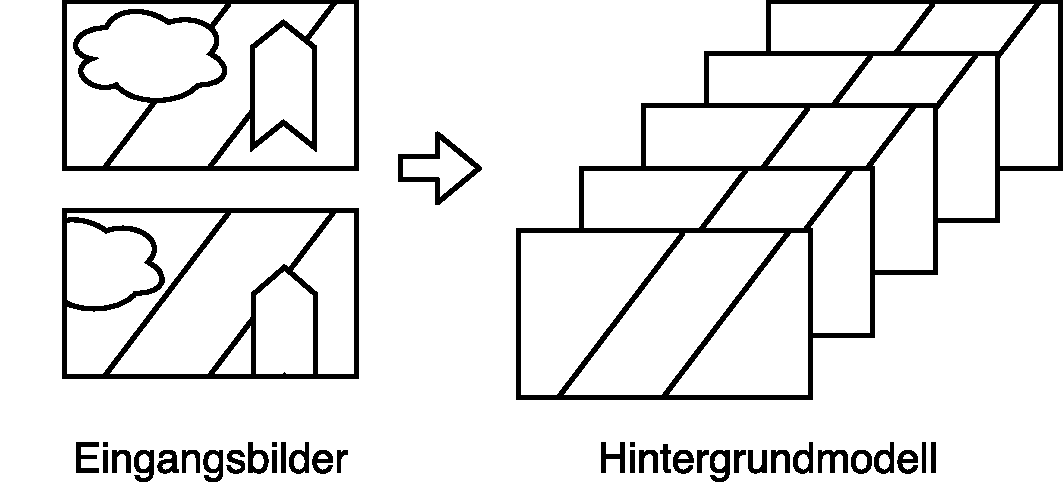
\includegraphics[width=0.95\linewidth]{Abbildungen/modell.pdf}
		\label{fig:Abbildungen/Grid}
	\end{figure}
\end{frame}

\begin{frame}[t]{Hintergrundmodell -- Beispiel}
	\bigskip
	\bigskip
	\begin{figure}% 
		\centering
		\begin{minipage}{0.35\linewidth}
			\centering
			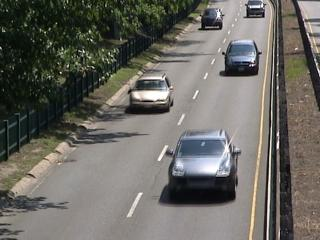
\includegraphics[width=0.8\linewidth]{Abbildungen/Eingang1.jpg}\\
			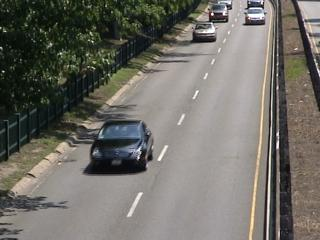
\includegraphics[width=0.8\linewidth]{Abbildungen/Eingang2.jpg}
			\caption*{Eingangsbilder}
		\end{minipage}
		\begin{minipage}{0.08\linewidth}
			\centering
			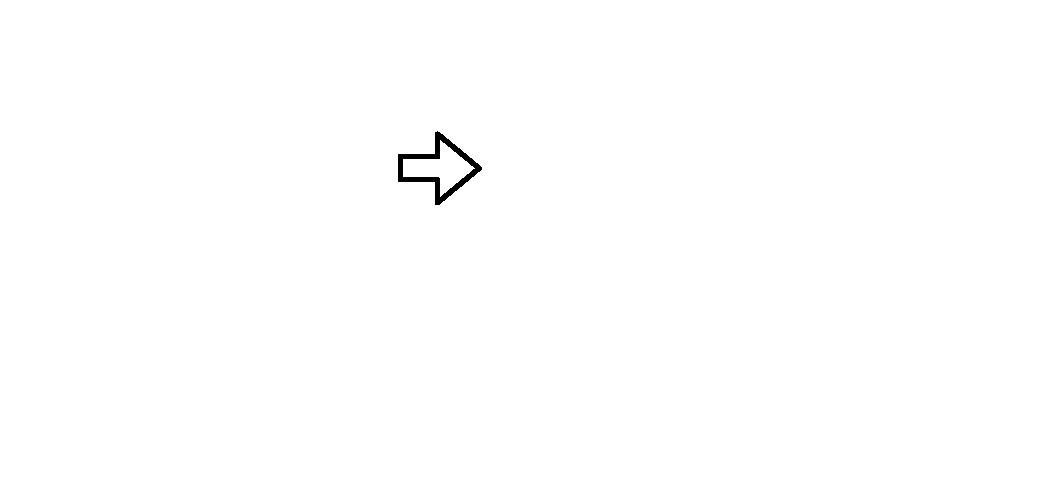
\includegraphics[width=0.8\linewidth]{Abbildungen/Pfeil.pdf}
		\end{minipage}
		\begin{minipage}{0.45\linewidth}
			\centering
			\begin{tikzpicture}[scale=0.5]
				\node(5) at (2,3) {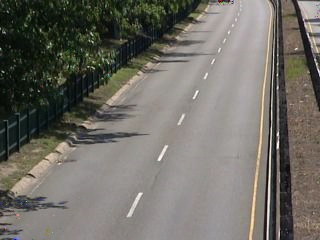
\includegraphics[width=0.7\linewidth]{Abbildungen/Hintergrund.jpg}};
				\node(4) at (1,2) {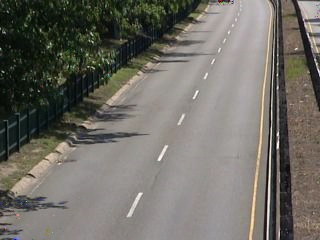
\includegraphics[width=0.7\linewidth]{Abbildungen/Hintergrund.jpg}};
				\node(3) at (0,1.5) {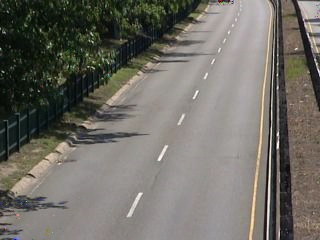
\includegraphics[width=0.7\linewidth]{Abbildungen/Hintergrund.jpg}};
				\node(2) at (-1,0.5) {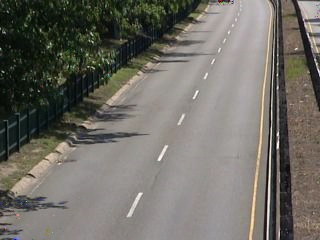
\includegraphics[width=0.7\linewidth]{Abbildungen/Hintergrund.jpg}};
				\node(1) at (-2,-0.5) {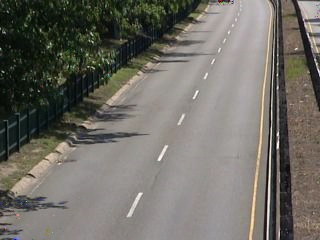
\includegraphics[width=0.7\linewidth]{Abbildungen/Hintergrund.jpg}};
			\end{tikzpicture}
			\caption*{Hintergrundmodell}
		\end{minipage}
	\end{figure}
\end{frame}



\begin{frame}[t]{Konzept des Algorithmus}
	\bigskip
	\bigskip
	\bigskip 
	\begin{figure}
		\centering
		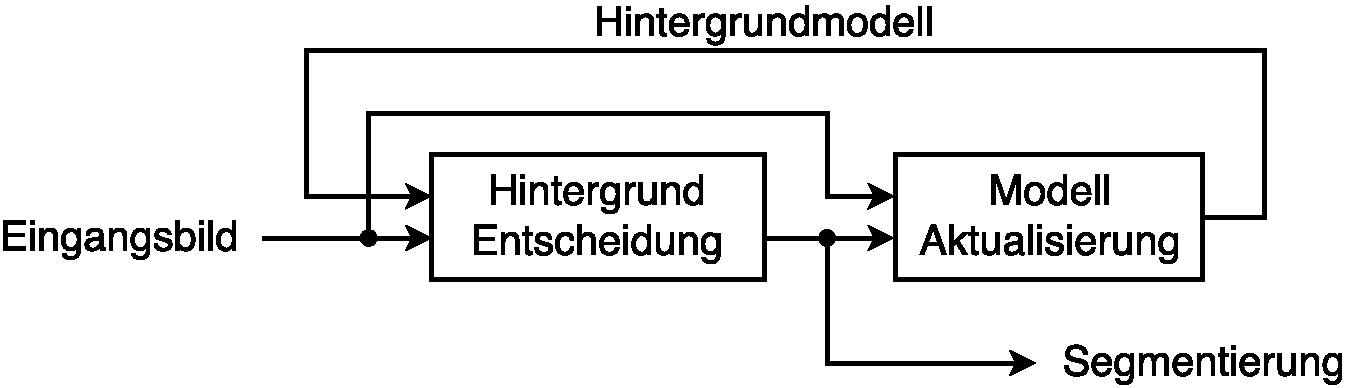
\includegraphics[width=1\linewidth]{Abbildungen/gesamt.pdf}
		\label{fig:Abbildungen/Grid}
	\end{figure}
\end{frame}


\begin{frame}[t]{Aktualisierung des Modells -- Hintergrund Dynamik}
	\vspace{1.65em}
	\begin{figure}
		\centering
		\begin{minipage}{0.45\linewidth}
			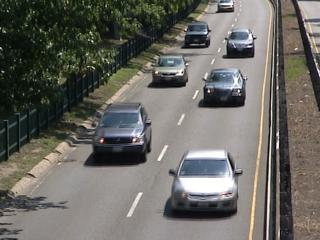
\includegraphics[width=1\linewidth]{Abbildungen/Eingang3.jpg}
			\caption*{Eingangsbild}
		\end{minipage}
		\begin{minipage}{0.45\linewidth}
			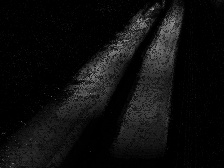
\includegraphics[width=1\linewidth]{Abbildungen/distance.jpg}
			\caption*{Hintergrund Dynamik}
		\end{minipage}
	\end{figure}
	\bigskip
	\begin{equation*}
		D_{min}(x) = D_{min}(x) \cdot (1-\alpha) + d_t(x) \cdot \alpha
	\end{equation*}
\end{frame}

\begin{frame}[t]{Aktualisierung des Modells -- Blinkende Pixel}
	\vspace{1.65em}
	\begin{figure}
		\centering
		\begin{minipage}{0.45\linewidth}
			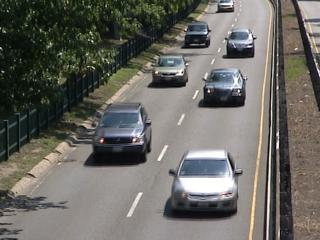
\includegraphics[width=1\linewidth]{Abbildungen/Eingang3.jpg}
			\caption*{Eingangsbild}
		\end{minipage}
		\begin{minipage}{0.45\linewidth}
			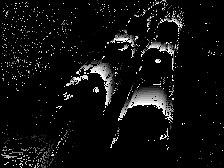
\includegraphics[width=1\linewidth]{Abbildungen/blinking_pixels1.jpg}
			\caption*{Blinkende Pixel}
		\end{minipage}
	\end{figure}
	\bigskip
	\begin{equation*}
		v(x)= 	\left\{
				\begin{array}{ll} 
					v(x) + v_{incr}, &  X(t) \oplus X(t-1) \\
					v(x) - v_{decr}, & sonst
				\end{array}
			\right .
	\end{equation*}
\end{frame}

\begin{frame}[t]{Aktualisierung des Modells -- Schwellwert}
	\vspace{1.65em}
	\begin{figure}
		\centering
		\begin{minipage}{0.45\linewidth}
			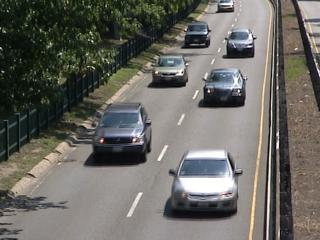
\includegraphics[width=1\linewidth]{Abbildungen/Eingang3.jpg}
			\caption*{Eingangsbild}
		\end{minipage}
		\begin{minipage}{0.45\linewidth}
			
\includegraphics[width=1\linewidth]{Abbildungen/R.jpg}
			\caption*{Schwellwert}
		\end{minipage}
	\end{figure}
	\bigskip
	\begin{equation*}
		R(x)= 	\left\{
				\begin{array}{ll} 
					R(x) + v(x), &  R(x) < (1 + D_{min}(x) \cdot 2)^2 \\
					R(x) - \frac{1}{v(x)}, & sonst
				\end{array}
			\right .
	\end{equation*}
\end{frame}

\begin{frame}[t]{Aktualisierung des Modells -- Schwellwert für den Farbvergleich}
	\begin{figure}
		\centering
		\begin{minipage}{0.45\linewidth}
			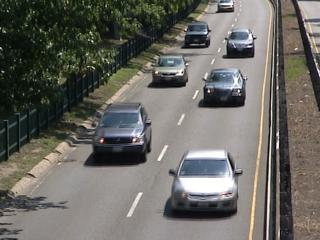
\includegraphics[width=1\linewidth]{Abbildungen/Eingang3.jpg}
			\caption*{Eingangsbild}
		\end{minipage}
		\begin{minipage}{0.45\linewidth}
			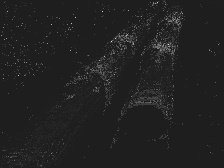
\includegraphics[width=1\linewidth]{Abbildungen/R_color.jpg}
			\caption*{Schwellwert}
		\end{minipage}
	\end{figure}
	\bigskip
	\begin{equation*}
		R_{color}(x) = R(x) \cdot R^0_{color} 	
	\end{equation*}
\end{frame}

\begin{frame}[t]{Aktualisierung des Modells -- Schwellwert für LBSP}
	\vspace{1.65em}
	\begin{figure}
		\centering
		\begin{minipage}{0.45\linewidth}
			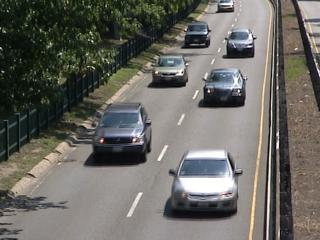
\includegraphics[width=1\linewidth]{Abbildungen/Eingang3.jpg}
			\caption*{Eingangsbild}
		\end{minipage}
		\begin{minipage}{0.45\linewidth}
			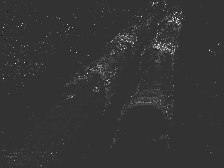
\includegraphics[width=1\linewidth]{Abbildungen/R_lbsp.jpg}
			\caption*{Schwellwert}
		\end{minipage}
	\end{figure}
	\bigskip
	\begin{equation*}
		R_{lbsp}(x) = 2^{R(x)} + R^0_{lbsp} 	
	\end{equation*}
\end{frame}

\begin{frame}[t]{Aktualisierung des Modells -- Wahrscheinlichkeit}
	\vspace{1.65em}
	\begin{figure}
		\centering
		\begin{minipage}{0.45\linewidth}
			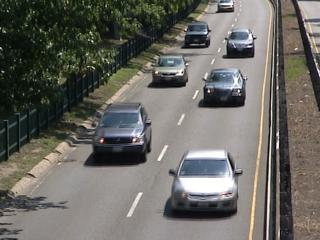
\includegraphics[width=1\linewidth]{Abbildungen/Eingang3.jpg}
			\caption*{Eingangsbild}
		\end{minipage}
		\begin{minipage}{0.45\linewidth}
			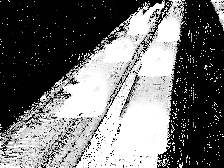
\includegraphics[width=1\linewidth]{Abbildungen/threshold.jpg}
			\caption*{Schwellwert}
		\end{minipage}
	\end{figure}
	\bigskip
	\begin{equation*}
		T(x)= 	\left\{
				\begin{array}{ll} 
					T(x) + \frac{1}{v(x)\cdot D_{min}(x)}, &  S_t(x) = 1 \\
					T(x) + \frac{v(x)}{D_{min}(x)}, &  S_t(x) = 0 \\
				\end{array}
			\right .
	\end{equation*}
\end{frame}

\begin{frame}[t]{Aktualisierung des Modells -- Aktualisierung}
	\vspace{1.65em}
	\begin{figure}
		\centering
		\begin{minipage}{0.45\linewidth}
			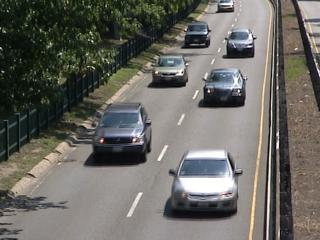
\includegraphics[width=1\linewidth]{Abbildungen/Eingang3.jpg}
			\caption*{Eingangsbild}
		\end{minipage}
		\begin{minipage}{0.45\linewidth}
			
\includegraphics[width=1\linewidth]{Abbildungen/update_array.jpg}
			\caption*{Aktualisierungsarray}
		\end{minipage}
	\end{figure}
\end{frame}

\begin{frame}[t]{Gesamtalgorithmus -- Beispiel}
	\vspace{1.65em}
	\begin{figure}
		\centering
		\begin{minipage}{0.45\linewidth}
			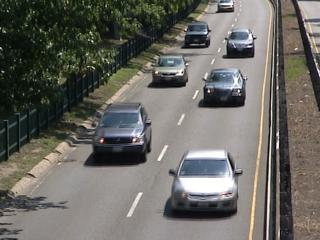
\includegraphics[width=1\linewidth]{Abbildungen/Eingang3.jpg}
			\caption*{Eingangsbild}
		\end{minipage}
		\begin{minipage}{0.45\linewidth}
			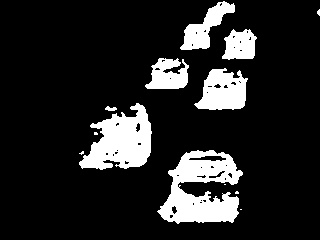
\includegraphics[width=1\linewidth]{Abbildungen/Segmentierung.jpg}
			\caption*{Gesamtsegmentierung}
		\end{minipage}
	\end{figure}
\end{frame}


\title{Pixel-Based Adaptive Segmenter}   
\author{Christian Tanzer} 
\date{}

\section{Pixel-Based Adaptive Segmenter}

\begin{frame}
	\maketitle
\end{frame}




\section{Vergleich}

\title{Vergleich SuBSENSE und PBAS}   
\author{} 
\date{}


\begin{frame}
	\maketitle
\end{frame}


\begin{frame}[t]{Vergleich -- Precision}
	\begin{equation*}
		Pr = \frac{TP}{TP+FP}
	\end{equation*}

	\begin{figure}[htpb]
		\centering
		\begin{tikzpicture}
			\begin{axis}[ylabel = {Pr},ymajorgrids = true,symbolic x coords={SuBSENSE,PBAS},xtick=data,ymin = 0.5,bar width=14pt, ymax = 1, axis x line=middle, axis y line=left, enlarge x limits=1, height = 6 cm]
			    \addplot[ybar,fill=blue] coordinates {
				(SuBSENSE,0.858)
				(PBAS,0.816)
			    };
			\end{axis}
		\end{tikzpicture}
	\end{figure}
	
\end{frame}


\begin{frame}[t]{Vergleich -- Recall}
	\begin{equation*}
		Re = \frac{TP}{TP+FN}
	\end{equation*}

	\begin{figure}[htpb]
		\centering
		\begin{tikzpicture}
		       \begin{axis}[ylabel = {Re},ymajorgrids = true,symbolic x coords={SuBSENSE,PBAS},xtick=data,ymin = 0.5,bar width=14pt, ymax = 1, axis x line=middle, axis y line=left, enlarge x limits=1, height = 6 cm]
			    \addplot[ybar,fill=blue] coordinates {
				(SuBSENSE,0.828)
				(PBAS,0.784)
			    };
			\end{axis}
		\end{tikzpicture}
	\end{figure}
	
\end{frame}

\begin{frame}[t]{Vergleich -- Accuracy}
	\begin{equation*}
		FM = \frac{2 \cdot Pr \cdot Re}{Pr + Re}
	\end{equation*}

	\begin{figure}[htpb]
		\centering
		\begin{tikzpicture}
		       \begin{axis}[ylabel = {FM},ymajorgrids = true,symbolic x coords={SuBSENSE,PBAS},xtick=data,ymin = 0.5,bar width=14pt, ymax = 1, axis x line=middle, axis y line=left, enlarge x limits=1, height = 6 cm]
			    \addplot[ybar,fill=blue] coordinates {
				(SuBSENSE,0.826)
				(PBAS,0.753)
			    };
			\end{axis}
		\end{tikzpicture}
	\end{figure}
	
\end{frame}

\begin{frame}[t]{Vergleich -- Accuracy}

	\begin{figure}[htpb]
		\centering
		\begin{tikzpicture}
		       \begin{axis}[
				width  = 1*\textwidth,
				height = 5.5cm,
				major x tick style = transparent,
				ybar=2*\pgflinewidth,
				bar width=14pt,
				ymajorgrids = true,
				ylabel = {FM},
				symbolic x coords={baseline,camera jitter, dyn. backgr.,shadow, thermal},
				xtick = data,
				x tick label style={rotate=45,anchor=east},
				scaled y ticks = false,
				enlarge x limits=0.25,
				ymin=0,
				legend cell align=left,
				legend style={
					at={(1,1.03)},
					anchor=south east,
					column sep=1ex}
				]				
				
				\addplot[ybar,fill=green] 
					coordinates {(baseline,0.95)(camera jitter,0.815)(dyn. backgr., 0.818)(shadow,0.899)(thermal,0.817)};
				\addlegendentry{SuBSENSE}
				\addplot[ybar,fill=blue]
					coordinates {(baseline,0.924)(camera jitter,0.722)(dyn. backgr., 0.683)(shadow,0.86)(thermal,0.756)};
				\addlegendentry{PBAS}

			\end{axis}
		\end{tikzpicture}
	\end{figure}
	
\end{frame}



\begin{frame}[t]{Quellen}
	\begin{itemize}
		\item \url{http://www.stern.de/kultur/photoshop-oder-bodypainting--der-kuenstler-liu-bolin-macht-menschen-unsichtbar-6618586.html}, aufgerufen am 1. Dezember 2016
		\item \url{http://www.sueddeutsche.de/auto/autonomes-fahren-was-autonome-autos-koennen-und-was-nicht-1.3062258}, aufgerufen am 1. Dezember 2016
		\item Rafael C. Gonzalez, Richard E. Woods: "Digital Image Processing", Addison-Wesley Publishing Company, 1992
		\item Pierre-Luc St-Charles,Guillaume-Alexandre Bilodeau and Robert Bergevin: "SuBSENSE: A Universal Change Detection Method With Local Adaptive Sensitivity" in IEEE Transactions on Image Processing, vol. 24, no. 1, pp. 359-373, Januar 2015
	\end{itemize}
\end{frame}

\end{document}
